\Problem
{نحوه اجرای برنامه}
{
برای راحتی اجرای برنامه یک
\lr{Help}
ایجاد شده است که با زدن دستور زیر می‌توانیم آن را مشاهده کنیم.

\lr{python main.py -h}

\begin{figure}[H]
    \centering
    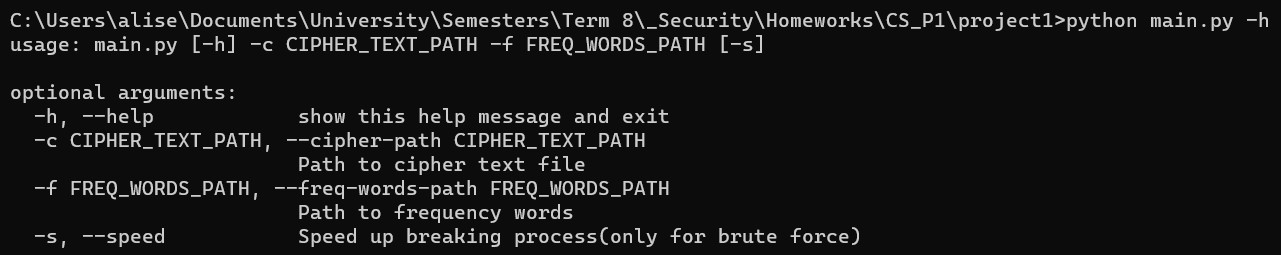
\includegraphics[width=15cm]{Images/Help.jpg}
    \label{fig:label}
    \caption{راهنمای اجرای برنامه}
\end{figure}

نمونه دستور برای اجرا برنامه:

\begin{latin}
    CLI Commands:\\
    python main.py -c cipher\_text.txt -f words-by-frequency.txt -s\\
    python main.py -c cipher\_text.txt -f words-by-frequency.txt\\
\end{latin}

دستور اول برای اسپیس‌گذاری از فایل کلمات پر تکرار استفاده می‌کند که روش سریع‌تری است.
دستور دوم از کتابخانه
\lr{wordninja}
برای فاصله‌گذاری صحیح میان کلمات استفاده می‌کند که نیازمند نصب بودن این کتابخانه است. این روش سرعت کمتری دارد.
}
